\documentclass[xcolor=dvipsnames]{beamer}
\usetheme{Madrid}
\useoutertheme{miniframes}
\useinnertheme{circles}
\definecolor{UBCblue}{rgb}{0.04706, 0.13725, 0.26667} %Allows us to change the beamer's color
\usecolortheme[named=UBCblue]{structure}

\usepackage{graphicx} % Allows to include images
\usepackage{booktabs} % Allows the use of \toprule, \midrule and \bottomrule in tables
%\usepackage{subcaption}
%\usepackage[demo]{graphicx}% delete the demo option in your actual code
%\usepackage{enumitem}
%\usepackage{booktabs}
%\usepackage{xcolor}
% --------------------------------------------------- %
%                    Title + Schedule                 %
% --------------------------------------------------- %
\title[Presentaci\'on]{El efecto traspaso del tipo de cambio a los precios de internet}
\subtitle[]{¿Efectos no lineales?}
\author{Alexandra Marcos}
\institute[PUCP]{Pontificia Universidad Catolica del Per\'u}
\date{\today}

% --------------------------------------------------- %
%                  Presentation info	              %
% --------------------------------------------------- %


\begin{document}

\begin{frame}
\titlepage
\end{frame}

\begin{frame}{Esquema de presentaci\'on}
  \tableofcontents
\end{frame}

\section{Revision de la Literatura}
\begin{frame}
Revision de la literatura
\end{frame}

\begin{frame}
\begin{description}[font=$\bullet$~\normalfont\scshape\color{red!50!black}]
\item [$\bullet$ Importancia del ERPT]
\item [$\bullet$ Precio offline]
\end{description}
\end{frame}

\begin{frame}
\begin{description}[font=$\bullet$~\normalfont\scshape\color{red!50!black}]
\item [$\bullet$ Precion onlines]
\item [$\bullet$ Efectos no lineales]
\end{description}
\end{frame}

\section{Descripci\'on de la base de datos}
\begin{frame}
Descripci\'on de la base de datos
\end{frame}
\begin{frame}
Base de datos en formato panel
\begin{enumerate}[I]
\item Periodo de estudio
\begin{enumerate}[i]
  \item Inicio: 2016-09-19
  \item Final: 2019-04-30
\end{enumerate}
\item Clasificaci\'on de los productos (Categor\'ias)
%\item [$\bullet$ Bienes "ID" ] 1272
\begin{enumerate}[i]
  \item Audio
  \item Computadores
  \item Electrodom\'estico
  \item Fotograf\'ia
  \item Linea Blanca
  \item Tecnolog\'ia
  \item Tel\'efonos
  \item Televisores
  \item Electrohogar
\end{enumerate}
\item N\'umero de productos (ID): 1272
\end{enumerate}
\end{frame}

\begin{frame}
Observaciones por categor\'ia
\centering
\begin{tabular}{lrrr}
\toprule
categoria & n & observaciones & obs\_item\\
\midrule
audio & 21 & 5 712 & 272\\
computadores & 61 & 16 841 & 276\\
electrodom\'esticos & 86 & 24 281 & 282\\
electrohogar & 598 & 195 988 & 328\\
fotograf\'ia & 19 & 5 467 & 288\\
\addlinespace
linea blanca & 85 & 23 988 & 282\\
tecnolog\'ia & 301 & 96 584 & 321\\
tel\'efonos & 72 & 20 838 & 289\\
televisores & 29 & 8 654 & 298\\
\bottomrule
\end{tabular}
\end{frame}

\begin{frame}
Histograma del n\'umero de observaciones por ID
\begin{figure}
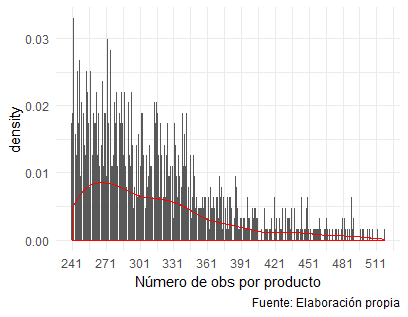
\includegraphics[scale=0.75]{observaciones_producto.png}
\caption{Figura 1}
\end{figure}
\end{frame}

\begin{frame}
Grafico de densidad del n\'umero de observaciones por categoria
\begin{figure}
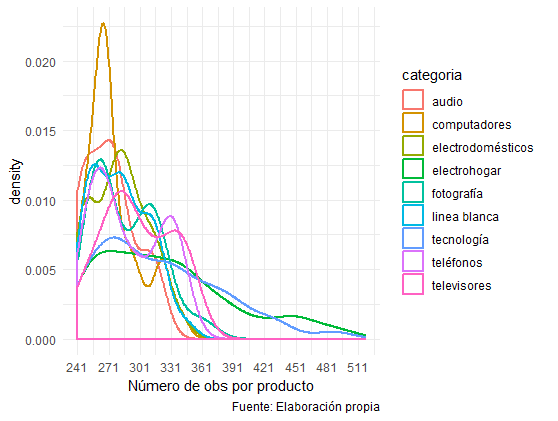
\includegraphics[scale=0.60]{observaciones_categoria.png}
\caption{Figura 2}
\end{figure}
\end{frame}


\begin{frame}
Porcentaje de observaciones por ID
\begin{figure}
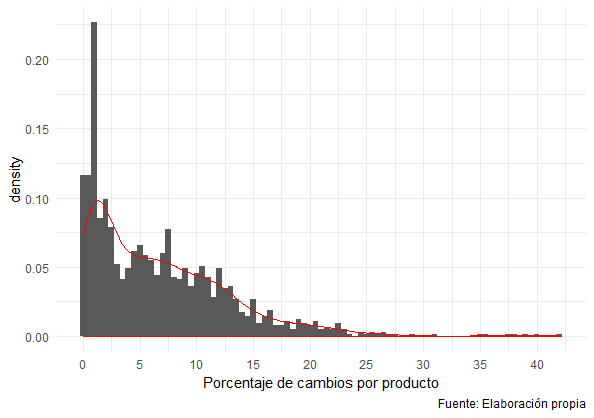
\includegraphics[scale=0.60]{cambio_producto.png}
\caption{Figura 3}
\end{figure}
\end{frame}


\begin{frame}
Porcentaje de observaciones por ID
\centering
\begin{tabular}{rrrrrr}
\toprule
Min & Q1 & Median & Mean & Q3 & Max\\
\midrule
0 & 1.542917 & 5.353921 & 6.722289 & 10.28881 & 42.14286\\
\bottomrule
\end{tabular}
%\caption{\label{tab:table-name}Your caption.}
\end{frame}



\begin{frame}
Frecuencia de cambios por dia
\begin{figure}
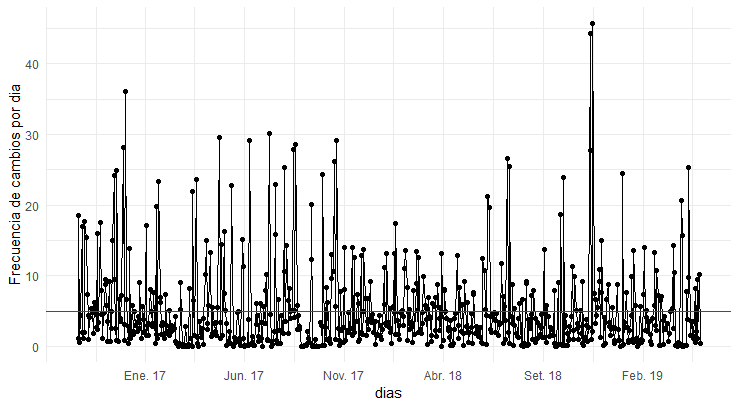
\includegraphics[scale=0.60]{frecuencia_dias.png}
\caption{4}
\end{figure}
\end{frame}

%\begin{frame}
%Frecuencia de cambios promedio mensual
%\begin{figure}
%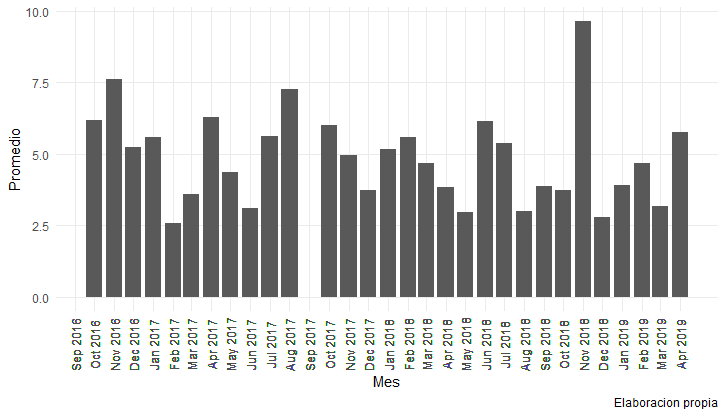
\includegraphics[scale=0.60]{frecuencia_mensual.png}
%\caption{5}
%\end{figure}
%\end{frame}

\begin{frame}
Tamaño del cambio promedio por d\'ia
\begin{figure}
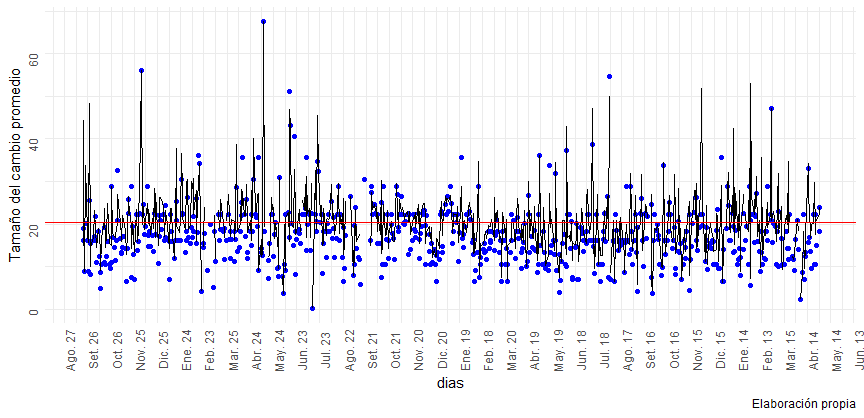
\includegraphics[scale=0.50]{tamano_cambio_promedio.png}
\caption{Figura 6}
\end{figure}
\end{frame}


\section{Descripci\'on de la base de duraciones}

\begin{frame}
Descripci\'on de la base de duraciones
\end{frame}


\begin{frame}
Duraci\'on de precio para toda la base
\centering
\begin{tabular}{rrr}
\toprule
 & Con censura manual (meses) & Sin censura manual (meses)\\
\midrule
Promedio & 1.457289 & 0.75 \\ Mediana & 1.154425 & 0.70\\
\bottomrule
\end{tabular}
\end{frame}

\begin{frame}

\centering
Duraci\'on de precios por categoria (sin censura manual)
\begin{tabular}{lrr}
\toprule
categoria & mean & median\\
\midrule
audio & 5.069000 & 1.750\\
computadores & 3.014943 & 1.225\\
electrodomésticos & 1.687437 & 0.850\\
electrohogar & 1.222188 & 0.700\\
fotografía & 1.539015 & 0.750\\
\addlinespace
linea blanca & 1.575000 & 0.700\\
tecnología & 1.857261 & 0.750\\
teléfonos & 2.293314 & 0.900\\
televisores & 1.736829 & 0.650\\
\bottomrule
\end{tabular}
\end{frame}

\begin{frame}
Duracion de precios por categoria (con censura manual)
\centering
\begin{tabular}{lrr}
\toprule
categoria & mean & median\\
\midrule
audio & 1.732258 & 0.85\\
computadores & 2.628512 & 1.05\\
electrodomésticos & 1.269809 & 0.80\\
electrohogar & 1.043629 & 0.70\\
fotografía & 1.474576 & 0.80\\
\addlinespace
linea blanca & 1.151814 & 0.65\\
tecnología & 1.375224 & 0.70\\
teléfonos & 1.639426 & 0.75\\
televisores & 1.070506 & 0.65\\
\bottomrule
\end{tabular}
\end{frame}

\begin{frame}
N\'umero de observaciones por categoria\\
\centering
\begin{tabular}{lr}
\toprule
categoria & n\\
\midrule
audio & 50\\
computadores & 174\\
electrodomésticos & 796\\
electrohogar & 8820\\
fotografía & 132\\
\addlinespace
linea blanca & 754\\
tecnología & 2486\\
teléfonos & 344\\
televisores & 205\\
\bottomrule
\end{tabular}
\end{frame}

\begin{frame}
Distribuci\'on e histograma de los cambios de precios.
\begin{figure}
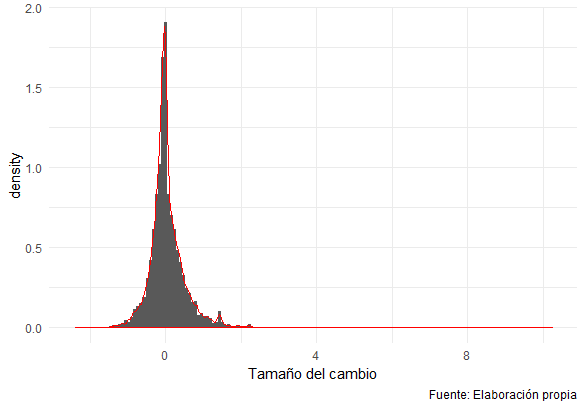
\includegraphics[scale=0.50]{cambios_precios_duraciones.png}
%\caption{7}
\end{figure}
\end{frame}


\begin{frame}
\begin{table}[h]
\begin{tabular}{cc}
Apreciaci\'on & Depreciaci\'on \\
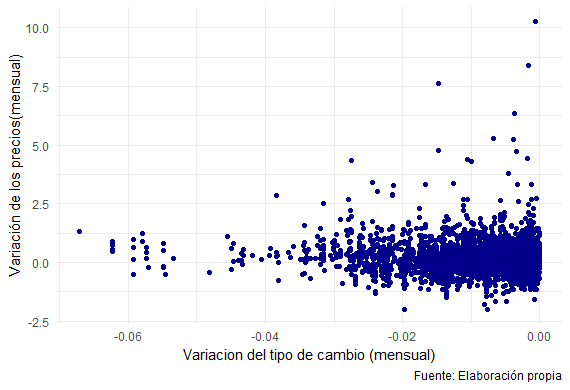
\includegraphics[height=3.99cm, scale = 1.0]{apreciacion.png} &
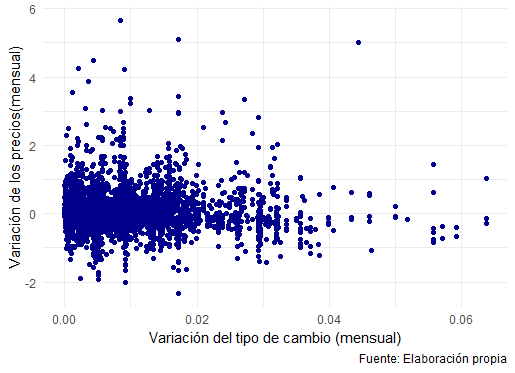
\includegraphics[height=3.99cm, scale =1.0]{depreciacion.png} \\
\end{tabular}
\end{table}
\end{frame}

\begin{frame}
Grafico de dispersion
\begin{figure}
  \centering
  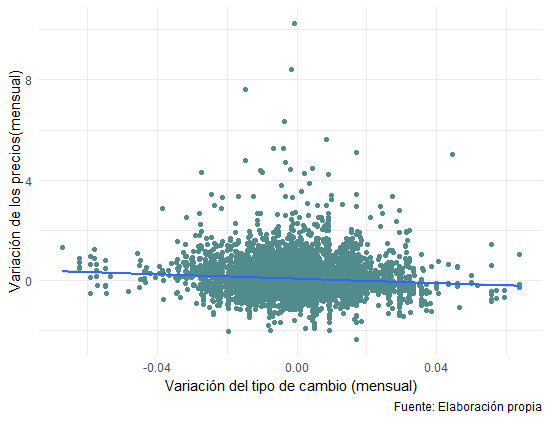
\includegraphics[scale=0.60]{grafico_dispersion.png}
  %\caption{}\label{}
\end{figure}
\end{frame}

\section{Modelo Econom\'etrico}

\begin{frame}
Modelo econom\'etrico
\end{frame}

\begin{frame}
\begin{equation}
  \Delta P_{t} = \beta_{1} \Delta ER_{t} + \beta_{2} {dummies categoria} + \varepsilon_{t}
\end{equation}
\begin{table}[!htbp] \centering
  \caption{}
  \label{}
\begin{tabular}{@{\extracolsep{5pt}}lD{.}{.}{-3} }
\\[-1.8ex]\hline
\hline \\[-1.8ex]
 & \multicolumn{1}{c}{\textit{Dependent variable:}} \\
\cline{2-2}
\\[-1.8ex] & \multicolumn{1}{c}{Dpre\_m} \\
\hline \\[-1.8ex]
 dER\_m & -4.420^{***} \\
  & (0.435) \\
  & \\
  dummies & SI & \\
\hline \\[-1.8ex]
Observations & \multicolumn{1}{c}{12,655} \\
R$^{2}$ & \multicolumn{1}{c}{0.022} \\
Adjusted R$^{2}$ & \multicolumn{1}{c}{0.022} \\
Residual Std. Error & \multicolumn{1}{c}{0.548 (df = 12645)} \\
F Statistic & \multicolumn{1}{c}{28.844$^{***}$ (df = 10; 12645)} \\
\hline
\hline \\[-1.8ex]
\textit{Note:}  & \multicolumn{1}{r}{$^{*}$p$<$0.1; $^{**}$p$<$0.05; $^{***}$p$<$0.01} \\
\end{tabular}
\end{table}
\end{frame}

\begin{frame}
\begin{equation}
  \Delta P_{t} = \beta_{1} \Delta ER_{t} + \beta_{2} A_{t} + \beta_{3} D_{t}+ \varepsilon_{t}
\end{equation}
\begin{table}[!htbp] \centering
\small\addtolength{\tabcolsep}{-15pt}
\begin{tabular}{@{\extracolsep{5pt}}lc}
\\[-1.8ex]\hline
\hline \\[-1.8ex]
 & \multicolumn{1}{c}{\textit{Dependent variable:}} \\
\cline{2-2}
\\[-1.8ex] & Dpre\_m \\
\hline \\[-1.8ex]
 dER\_m & $-$5.538$^{***}$ \\
  & (0.617) \\
 A & 0.046$^{***}$ \\
  & (0.008) \\
 D & 0.082$^{***}$ \\
  & (0.009) \\
\hline \\[-1.8ex]
Observations & 12,655 \\
R$^{2}$ & 0.021 \\
Adjusted R$^{2}$ & 0.021  \\
F Statistic & 90.479$^{***}$ (df = 3; 12652) \\
\hline
\hline \\[-1.8ex]
\textit{Note:}  & \multicolumn{1}{r}{$^{*}$p$<$0.1; $^{**}$p$<$0.05; $^{***}$p$<$0.01} \\
\end{tabular}
\end{table}
\end{frame}


\begin{frame}
\begin{equation}
\Delta P_{t} = \beta_{1} \Delta ER_{t} + \beta_{2} L_{t} + \beta_{3} S_{t} + \varepsilon_{t}
\end{equation}
\begin{table}[!htbp] \centering
\small\addtolength{\tabcolsep}{-15pt}
\begin{tabular}{@{\extracolsep{5pt}}lc}
\\[-1.8ex]\hline
\hline \\[-1.8ex]
 & \multicolumn{1}{c}{\textit{Dependent variable:}} \\
\cline{2-2}
\\[-1.8ex] & Dpre\_m \\
\hline \\[-1.8ex]
 dER\_m & $-$4.442$^{***}$ \\
  & (0.436) \\
 L & 0.102$^{***}$ \\
  & (0.034) \\
 S & 0.063$^{***}$ \\
  & (0.005) \\
\hline \\[-1.8ex]
Observations & 12,655 \\
R$^{2}$ & 0.021 \\
Adjusted R$^{2}$ & 0.020 \\
Residual Std. Error & 0.549 (df = 12652) \\
F Statistic & 88.678$^{***}$ (df = 3; 12652) \\
\hline
\hline \\[-1.8ex]
\textit{Note:}  & \multicolumn{1}{r}{$^{*}$p$<$0.1; $^{**}$p$<$0.05; $^{***}$p$<$0.01} \\
\end{tabular}
\end{table}
\end{frame}

\begin{frame}
\begin{equation}
\Delta P_{t} = \beta_{0} + \beta_{1} I(1/ \Delta ER_{t})  + \varepsilon_{t}
\end{equation}
\begin{table}[!htbp] \centering
\begin{tabular}{@{\extracolsep{5pt}}lc}
\\[-1.8ex]\hline
\hline \\[-1.8ex]
 & \multicolumn{1}{c}{\textit{Dependent variable:}} \\
\cline{2-2}
\\[-1.8ex] & abs(Dpre\_m) \\
\hline \\[-1.8ex]
 I(1/abs\_tc) & $-$0.00001$^{***}$ \\
  & (0.00000) \\
 Constant & 0.354$^{***}$ \\
  & (0.004) \\
\hline \\[-1.8ex]
Observations & 12,655 \\
R$^{2}$ & 0.002 \\
Adjusted R$^{2}$ & 0.002 \\
Residual Std. Error & 0.429 (df = 12653) \\
F Statistic & 25.190$^{***}$ (df = 1; 12653) \\
\hline
\hline \\[-1.8ex]
\textit{Note:}  & \multicolumn{1}{r}{$^{*}$p$<$0.1; $^{**}$p$<$0.05; $^{***}$p$<$0.01} \\
\end{tabular}
\end{table}
\end{frame}

\end{document} 